\documentclass{standalone}
\usepackage{tikz}
\usetikzlibrary{patterns, positioning}

\begin{document}
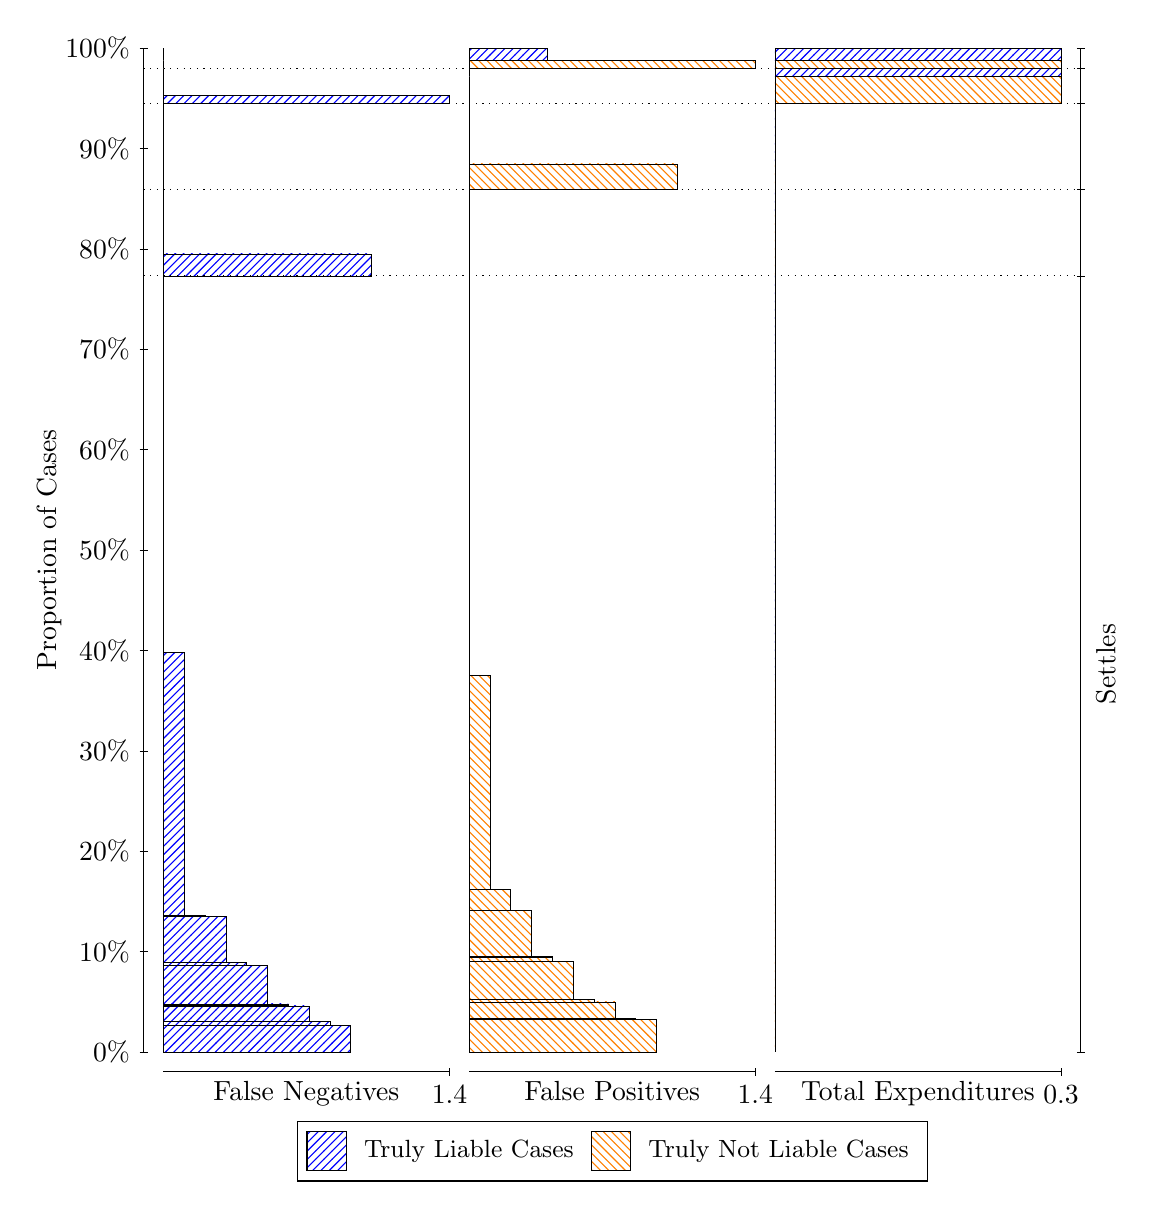
\begin{tikzpicture}
\draw[black, very thin] (1.5,1.75) -- (1.5,14.5);
\node[rotate=90, anchor=center] at (0.3, 8.125) {Proportion of Cases};
\draw[black, very thin] (1.45,1.75) -- (1.55,1.75);
\node[anchor=east] at (1.45, 1.75) {0\%};
\draw[black, very thin] (1.45,3.025) -- (1.55,3.025);
\node[anchor=east] at (1.45, 3.025) {10\%};
\draw[black, very thin] (1.45,4.3) -- (1.55,4.3);
\node[anchor=east] at (1.45, 4.3) {20\%};
\draw[black, very thin] (1.45,5.575) -- (1.55,5.575);
\node[anchor=east] at (1.45, 5.575) {30\%};
\draw[black, very thin] (1.45,6.85) -- (1.55,6.85);
\node[anchor=east] at (1.45, 6.85) {40\%};
\draw[black, very thin] (1.45,8.125) -- (1.55,8.125);
\node[anchor=east] at (1.45, 8.125) {50\%};
\draw[black, very thin] (1.45,9.4) -- (1.55,9.4);
\node[anchor=east] at (1.45, 9.4) {60\%};
\draw[black, very thin] (1.45,10.675) -- (1.55,10.675);
\node[anchor=east] at (1.45, 10.675) {70\%};
\draw[black, very thin] (1.45,11.95) -- (1.55,11.95);
\node[anchor=east] at (1.45, 11.95) {80\%};
\draw[black, very thin] (1.45,13.225) -- (1.55,13.225);
\node[anchor=east] at (1.45, 13.225) {90\%};
\draw[black, very thin] (1.45,14.5) -- (1.55,14.5);
\node[anchor=east] at (1.45, 14.5) {100\%};

\draw[black, very thin] (13.4,1.75) -- (13.4,14.5);
\draw[black, very thin] (13.35,1.75) -- (13.45,1.75);
\node[anchor=west] at (13.35, 1.75) {};
\draw[black, very thin] (13.35,11.606) -- (13.45,11.606);
\node[anchor=west] at (13.35, 11.606) {};
\draw[black, very thin] (13.35,12.709) -- (13.45,12.709);
\node[anchor=west] at (13.35, 12.709) {};
\draw[black, very thin] (13.35,13.795) -- (13.45,13.795);
\node[anchor=west] at (13.35, 13.795) {};
\draw[black, very thin] (13.35,14.241) -- (13.45,14.241);
\node[anchor=west] at (13.35, 14.241) {};
\draw[black, very thin] (13.35,14.5) -- (13.45,14.5);
\node[anchor=west] at (13.35, 14.5) {};

\draw[black, very thin, pattern color=blue, pattern=north east lines] (1.75,1.75) rectangle (4.1282,2.0886);
\draw[black, very thin, pattern color=blue, pattern=north east lines] (1.75,2.0886) rectangle (3.8639,2.1336);
\draw[black, very thin, pattern color=blue, pattern=north east lines] (1.75,2.1336) rectangle (3.5997,2.3364);
\draw[black, very thin, pattern color=blue, pattern=north east lines] (1.75,2.3364) rectangle (3.3355,2.3386);
\draw[black, very thin, pattern color=blue, pattern=north east lines] (1.75,2.3386) rectangle (3.3355,2.3621);
\draw[black, very thin, pattern color=blue, pattern=north east lines] (1.75,2.3621) rectangle (3.0712,2.8485);
\draw[black, very thin, pattern color=blue, pattern=north east lines] (1.75,2.8485) rectangle (2.807,2.8865);
\draw[black, very thin, pattern color=blue, pattern=north east lines] (1.75,2.8865) rectangle (2.5427,3.4688);
\draw[black, very thin, pattern color=blue, pattern=north east lines] (1.75,3.4688) rectangle (2.2785,3.4886);
\draw[black, very thin, pattern color=blue, pattern=north east lines] (1.75,3.4886) rectangle (2.0142,6.8202);
\draw[black, very thin, pattern color=orange, pattern=north west lines] (1.75,6.8202) rectangle (1.75,11.606);
\draw[black, very thin, pattern color=blue, pattern=north east lines] (1.75,11.606) rectangle (4.3924,11.885);
\draw[black, very thin, pattern color=orange, pattern=north west lines] (1.75,11.885) rectangle (1.75,12.709);
\draw[black, very thin, pattern color=orange, pattern=north west lines] (1.75,12.709) rectangle (1.75,13.029);
\draw[black, very thin, pattern color=blue, pattern=north east lines] (1.75,13.029) rectangle (1.75,13.795);
\draw[black, very thin, pattern color=blue, pattern=north east lines] (1.75,13.795) rectangle (5.3833,13.897);
\draw[black, very thin, pattern color=orange, pattern=north west lines] (1.75,13.897) rectangle (1.75,14.241);
\draw[black, very thin, pattern color=orange, pattern=north west lines] (1.75,14.241) rectangle (1.75,14.343);
\draw[black, very thin, pattern color=blue, pattern=north east lines] (1.75,14.343) rectangle (1.75,14.5);
\draw[black, very thin, pattern color=orange, pattern=north west lines] (5.6333,1.75) rectangle (8.0115,2.1662);
\draw[black, very thin, pattern color=orange, pattern=north west lines] (5.6333,2.1662) rectangle (7.7473,2.1754);
\draw[black, very thin, pattern color=orange, pattern=north west lines] (5.6333,2.1754) rectangle (7.483,2.385);
\draw[black, very thin, pattern color=orange, pattern=north west lines] (5.6333,2.385) rectangle (7.2188,2.4142);
\draw[black, very thin, pattern color=orange, pattern=north west lines] (5.6333,2.4142) rectangle (6.9545,2.9013);
\draw[black, very thin, pattern color=orange, pattern=north west lines] (5.6333,2.9013) rectangle (6.6903,2.9547);
\draw[black, very thin, pattern color=orange, pattern=north west lines] (5.6333,2.9547) rectangle (6.6903,2.9683);
\draw[black, very thin, pattern color=orange, pattern=north west lines] (5.6333,2.9683) rectangle (6.4261,3.5447);
\draw[black, very thin, pattern color=orange, pattern=north west lines] (5.6333,3.5447) rectangle (6.1618,3.8162);
\draw[black, very thin, pattern color=orange, pattern=north west lines] (5.6333,3.8162) rectangle (5.8976,6.5355);
\draw[black, very thin, pattern color=blue, pattern=north east lines] (5.6333,6.5355) rectangle (5.6333,11.606);
\draw[black, very thin, pattern color=orange, pattern=north west lines] (5.6333,11.606) rectangle (5.6333,12.429);
\draw[black, very thin, pattern color=blue, pattern=north east lines] (5.6333,12.429) rectangle (5.6333,12.709);
\draw[black, very thin, pattern color=orange, pattern=north west lines] (5.6333,12.709) rectangle (8.2758,13.029);
\draw[black, very thin, pattern color=blue, pattern=north east lines] (5.6333,13.029) rectangle (5.6333,13.795);
\draw[black, very thin, pattern color=orange, pattern=north west lines] (5.6333,13.795) rectangle (5.6333,14.138);
\draw[black, very thin, pattern color=blue, pattern=north east lines] (5.6333,14.138) rectangle (5.6333,14.241);
\draw[black, very thin, pattern color=orange, pattern=north west lines] (5.6333,14.241) rectangle (9.2667,14.343);
\draw[black, very thin, pattern color=blue, pattern=north east lines] (5.6333,14.343) rectangle (6.6242,14.5);
\draw[black, very thin, pattern color=orange, pattern=north west lines] (9.5167,1.75) rectangle (9.5167,6.5355);
\draw[black, very thin, pattern color=blue, pattern=north east lines] (9.5167,6.5355) rectangle (9.5167,11.606);
\draw[black, very thin, pattern color=orange, pattern=north west lines] (9.5167,11.606) rectangle (9.5167,12.429);
\draw[black, very thin, pattern color=blue, pattern=north east lines] (9.5167,12.429) rectangle (9.5167,12.709);
\draw[black, very thin, pattern color=orange, pattern=north west lines] (9.5167,12.709) rectangle (9.5167,13.029);
\draw[black, very thin, pattern color=blue, pattern=north east lines] (9.5167,13.029) rectangle (9.5167,13.795);
\draw[black, very thin, pattern color=orange, pattern=north west lines] (9.5167,13.795) rectangle (13.15,14.138);
\draw[black, very thin, pattern color=blue, pattern=north east lines] (9.5167,14.138) rectangle (13.15,14.241);
\draw[black, very thin, pattern color=orange, pattern=north west lines] (9.5167,14.241) rectangle (13.15,14.343);
\draw[black, very thin, pattern color=blue, pattern=north east lines] (9.5167,14.343) rectangle (13.15,14.5);
\draw[black, dotted] (1.5,11.606) -- (13.4,11.606);
\draw[black, dotted] (1.5,12.709) -- (13.4,12.709);
\draw[black, dotted] (1.5,13.795) -- (13.4,13.795);
\draw[black, dotted] (1.5,14.241) -- (13.4,14.241);
\draw[black, very thin] (1.75,1.5) -- (5.3833,1.5);
\node[anchor=north] at (3.5667, 1.5) {False Negatives};
\draw[black, very thin] (5.3833,1.45) -- (5.3833,1.55);
\node[anchor=north] at (5.3833, 1.45) {1.4};

\draw[black, very thin] (5.6333,1.5) -- (9.2667,1.5);
\node[anchor=north] at (7.45, 1.5) {False Positives};
\draw[black, very thin] (9.2667,1.45) -- (9.2667,1.55);
\node[anchor=north] at (9.2667, 1.45) {1.4};

\draw[black, very thin] (9.5167,1.5) -- (13.15,1.5);
\node[anchor=north] at (11.333, 1.5) {Total Expenditures};
\draw[black, very thin] (13.15,1.45) -- (13.15,1.55);
\node[anchor=north] at (13.15, 1.45) {0.3};

\node[black, centered, rotate=90] at (13.72, 6.6778) {Settles};





\draw (7.449999999999999,1.5) node[draw=none] (baseCoordinate) {};
\begin{scope}[align=center]
        \matrix[scale=0.5, draw=black, below=0.5cm of baseCoordinate, nodes={draw}, column sep=0.1cm]{
            \node[rectangle, draw, minimum width=0.5cm, minimum height=0.5cm, pattern=north east lines, pattern color=blue] {}; &
            \node[draw=none, font=\small] (B) {Truly Liable Cases}; &
            \node[rectangle, draw, minimum width=0.5cm, minimum height=0.5cm, pattern=north west lines, pattern color=orange] {}; &
            \node[draw=none, font=\small] (B) {Truly Not Liable Cases}; \\
            };
\end{scope}

\end{tikzpicture}
\end{document}